% REQUISITOS------------------------------------------------------------------

\section{ANÁLISE E PROJETO}
\label{chap:analise}
Esta seção apresenta os requisitos funcionais e não funcionais, a especificação dos requisitos funcionais, e os diagramas de caso de uso, classes e entidade-relacionamento.

\subsection{Requisitos Funcionais}
\label{sec:titSecReqFunc}

Os requisitos funcionais são artefatos gerados pela especificação de requisitos, que é o processo de escrever os requisitos de usuário e de sistema em um documento de requisitos. Preferencialmente, os requisitos de usuário e sistema devem ser claros, inequívocos, de fácil compreensão, completos e consistentes. Porém, na prática, é difícil que isso ocorra, visto que os envolvidos no processo veem os requisitos de formas diferentes, e em grande parte das vezes, nota-se conflitos e inconsistências relacionadas à esses requisitos \cite{Sommerville10}.

No presente projeto os requisitos foram obtidos com base na planilha de cálculo de correção e equilíbrio do solo, fornecida pelo cliente, utilizando a técnica de etnografia, que consiste em uma técnica de observação que pode ser usada na elicitação e análise de requisitos. O etnógrafo imerge no ambiente dos usuários e observa os hábitos de seu trabalho diário. Os requisitos de software podem ser deduzidos a partir dessas observações \cite{Sommerville10}.

\begin{landscape}
\begin{longtable}{|p{1.5cm}|p{5cm}|p{9cm}|p{2.5cm}|}
    \hline
    ID    & REQUISITO                                                                        & DESCRIÇÃO                                                                                                                                                                                                                                                                                               & PRIORIDADE \\\hline
    \endfirsthead
    %
    \hline
    ID    & REQUISITO                                                                        & DESCRIÇÃO                                                                                                                                                                                                                                                                                               & PRIORIDADE \\\hline
    \endhead
    %
    RF001 & Gerenciar informações da propriedade.                                            & O sistema deve permitir ao usuário cadastrar, remover, alterar ou listar informações do solo de um produtor.                                                                                                                                                                                            & Essencial  \\\hline
    RF002 & Gerenciar nutrientes do solo.                                                    & O sistema deve permitir ao usuário inserir, remover, alterar ou listar os nutrientes coletados na análise do solo.                                                                                                                                                                                      & Essencial  \\\hline
    RF003 & Exibir valores ideais.                                                           & O sistema deve exibir os valores ideais de cada teor inserido de acordo com a textura do solo.                                                                                                                                                                                                          & Importante \\\hline
    RF004 & Exibir valores dos nutrientes após correções.                                    & O sistema deve exibir os valores dos nutrientes inseridos após as correções.                                                                                                                                                                                                                            & Importante \\\hline
    RF005 & Gerenciar matéria orgânica.                                                      & O sistema deve permitir ao usuário inserir, remover, alterar ou listar o teor da matéria orgânica (M.O.) do solo.                                                                                                                                                                                       & Essencial  \\\hline
    RF006 & Exibir teor ideal da M.O.                                                        & O sistema deve exibir o teor ideal de matéria orgânica (M.O.).                                                                                                                                                                                                                                          & Importante \\\hline
    RF007 & Gerenciar dados relacionados à correção/recuperação  de Fósforo.                 & O sistema deve permitir ao usuário cadastrar, remover,  alterar ou listar valores ligados ao Fósforo, tais como teor a ser atingido, fonte a ser utilizada e eficiência.                                                                                                                                & Essencial  \\\hline
    RF008 & Exibir valores a serem aplicados no processo de correção/recuperação de Fósforo. & O sistema deve informar ao usuário a quantidade de Fósforo à ser aplicada assim como o seu custo.                                                                                                                                                                                                       & Importante \\\hline
    RF009 & Gerenciar valor/ton. (R\$) no processo relacionado às fontes de Fósforo.         & O sistema deve possibilitar ao usuário inserir, remover, alterar ou listar valores relacionados às fontes: superfosfato simples, superfosfato triplo, MAP, DAP, Yoorin, Fosfato Arad, Fosfato Gafsa, Fosfato Daoui, Fosfato  Patos Minas, Escória de Thomas, ácido Fosfórico e multifosfato magnesiano. & Essencial  \\\hline
    RF010 & Gerenciar dados relacionados à correção/recuperação do Potássio.                 & O sistema deve possibilitar ao usuário inserir, remover,  alterar ou listar dados relacionados à participação do Potássio na CTC assim como a fonte de Potássio a ser usada.                                                                                                                            & Essencial  \\\hline
    RF011 & Exibir valores relacionados à correção/recuperação do Potássio.                  & O sistema deve informar ao usuário dados à respeito do Potássio tais como: participação atual na CTC do solo,  participação do Potássio na CTC após correção, quantidade e custo a ser aplicada e sua participação ideal na CTC.                                                                        & Importante \\\hline
    RF012 & Gerenciar valor/ton. (R\$) no processo relacionado às fontes de Potássio.        & O sistema deve permitir ao usuário cadastrar, excluir, alterar ou listar valores como: cloreto de Potássio, Sulfato de Potássio e Sulfato de Potássio/Magnésio.                                                                                                                                         & Essencial  \\\hline
    RF013 & Cadastrar dados para a correção do cálcio e magnésio no solo                     & O sistema deve permitir o usuário informar dados acerca da correção do cálcio no solo.                                                                                                                                                                                                                  & Essencial \\\hline
    RF014 & Alterar dados para a correção do cálcio e magnésio no solo                       & O sistema deve permitir o usuário alterar os dados sobre a correção do solo.                                                                                                                                                                                                                            & Desejável  \\\hline
    RF015 & Exibir o teor de cálcio atualmente no solo                                       & O sistema deve apresentar ao usuário, o percentual de Cálcio na CTC atual (antes das correções)                                                                                                                                                                                                         & Essencial  \\\hline
    RF016 & Exibir o teor de cálcio ideal no solo                                            & O sistema deve apresentar ao usuário, o intervalo percentual de Cálcio ideal na CTC.                                                                                                                                                                                                                    & Importante  \\\hline
    RF017 & Calcular o percentual de cálcio ideal no solo                                    & O sistema deve apresentar ao usuário, o percentual ideal de Cálcio na CTC.                                                                                                                                                                                                                              & Importante  \\\hline
    RF018 & Exibir teor de magnésio atualmente no solo                                       & O sistema deve apresentar ao usuário o percentual de Magnésio atual na CTC.                                                                                                                                                                                                                             & Importante  \\\hline
    RF019 & Exibir o percentual ideal de magnésio no solo                                    & O sistema deve apresentar ao usuário o percentual de Magnésio ideal na CTC.                                                                                                                                                                                                                             & Importante  \\\hline
    RF020 & Exibir o valor do magnésio no solo após as correções                             & O sistema deve apresentar ao usuário o percentual de Magnésio na CTC após as correções.                                                                                                                                                                                                                 & Importante  \\\hline
    RF021 & Calcular o teor de magnésio no solo após as correções                            & O sistema deve calcular o percentual de Magnésio na CTC após as correções.                                                                                                                                                                                                                              & Importante  \\\hline
    RF022 & Exibir a quantidade de corretivo de cálcio e magnésio a ser aplicada no solo.    & O sistema deve exibir a quantidade a ser aplicada, em toneladas por hectare, do corretivo informado.                                                                                                                                                                                                    & Importante  \\\hline
    RF023 & Calcular a quantidade de corretivo a ser aplicada no solo.                       & O sistema deve calcular a quantidade a ser aplicada, em toneladas por hectare, do corretivo informado.                                                                                                                                                                                                  & Importante  \\\hline
    RF024 & Exibir a quantidade de enxofre que o corretivo fornecerá à terra                 & O sistema deve exibir o valor, em quilogramas por hectare, da quantidade de enxofre que o corretivo fornecerá.                                                                                                                                                                                          & Desejável  \\\hline
    RF025 & Exibir a quantidade de enxofre necessária                                        & O sistema deve exibir a quantidade suficiente, em quilogramas por hectare, da quantidade de enxofre necessária.                                                                                                                                                                                         & Desejável  \\\hline
    RF026 & Calcular e exibir o valor de V\% atual, ideal e após as correções                & O sistema deve calcular e exibir os valores de V\% atual, ideal e após as correções.                                                                                                                                                                                                                    & Importante  \\\hline
    \caption{Tabela de Requisitos Funcionais}
    \label{rf:tabela}
\end{longtable}
\end{landscape}

\clearpage

\begin{quadro}[!htb]
    \begin{tabular}{|p{3cm}|p{11cm}|}
        \hline
        \textbf{RS300} & \textbf{Cadastrar dados para a correção do cálcio e magnésio no solo} \\
        \hline
        Sumário        & O sistema deve permitir o usuário informar dados acerca da correção do cálcio no solo.                  \\
        \hline
        Pré-condições  & O usuário deve estar logado no sitema                  \\
        \hline
        Atores         & Usuário                  \\
        \hline
        Descrição      &
        \begin{itemize}
            \item Informa o percentual de cálcio desejado na CTC
            \item Seleciona qual fonte de cálcio será utilizada na correção
            \item Informa o custo médio em R\$/ha do corretivo
            \item Informa o percentual de PRNT do corretivo
            \item Informa o teor de CaO do corretivo
        \end{itemize}                 \\
        \hline
        Alternativas   &
        \begin{itemize}
            \item Caso o usuário não saiba o teor de CaO, será utilizado o valor médio do corretivo
        \end{itemize}                 \\
        \hline
        Exceção        &
        \begin{itemize}
            \item Caso o usuário informe um valor percental fora do intervalo de 0 a 100, não poderá proseguir com o preenchimento de outros campos.
            \item Caso o usuário informa um corretivo que não exista, uma mensagem de erro deverá ser exibida.
        \end{itemize}                   \\
        \hline
    \end{tabular}
\end{quadro}

\begin{quadro}[!htb]
    \begin{tabular}{|p{3cm}|p{11cm}|}
        \hline
        \textbf{RS301} & \textbf{Alterar dados para a correção do cálcio e magnésio no solo} \\
        \hline
        Sumário        & O sistema deve permitir o usuário alterar os dados sobre a correção do solo.                  \\
        \hline
        Pré-condições  & \begin{itemize}
            \item O usuário deve estar logado
            \item O usuário deverá acessar uma ??análise?? já existente 
        \end{itemize}                 \\
        \hline
        Atores         & Usuário                  \\
        \hline
        Descrição      &
        \begin{itemize}
            \item Informa o percentual de cálcio desejado na CTC
            \item Seleciona qual fonte de cálcio será utilizada na correção
            \item Informa o custo médio em R\$/ha do corretivo
            \item Informa o percentual de PRNT do corretivo
            \item Informa o teor de CaO do corretivo
        \end{itemize}                 \\
        \hline
        Alternativas   &
        \begin{itemize}
            \item Caso o usuário não saiba o teor de CaO, será utilizado o valor médio do corretivo
        \end{itemize}                 \\
        \hline
        Exceção        &
        \begin{itemize}
            \item Caso o usuário informe um valor percental fora do intervalo de 0 a 100, não poderá proseguir com o preenchimento de outros campos.
            \item Caso o usuário informe um corretivo que não exista, uma mensagem de erro deverá ser exibida.
        \end{itemize}                   \\
        \hline
    \end{tabular}
\end{quadro}

\begin{quadro}[!htb]
    \begin{tabular}{|p{3cm}|p{11cm}|}
        \hline
        \textbf{RS302} & \textbf{Alterar dados para a correção do cálcio e magnésio no solo} \\
        \hline
        Sumário        & O sistema deve permitir o usuário alterar os dados sobre a correção do solo.                  \\
        \hline
        Pré-condições  & \begin{itemize}
            \item O usuário deve estar logado
            \item O usuário deverá acessar uma ??análise?? já existente 
        \end{itemize}                 \\
        \hline
        Atores         & Usuário                  \\
        \hline
        Descrição      &
        \begin{itemize}
            \item Informa o percentual de cálcio desejado na CTC
            \item Seleciona qual fonte de cálcio será utilizada na correção
            \item Informa o custo médio em R\$/ha do corretivo
            \item Informa o percentual de PRNT do corretivo
            \item Informa o teor de CaO do corretivo
        \end{itemize}                 \\
        \hline
        Alternativas   &
        \begin{itemize}
            \item Caso o usuário não saiba o teor de CaO, será utilizado o valor médio do corretivo
        \end{itemize}                 \\
        \hline
        Exceção        &
        \begin{itemize}
            \item Caso o usuário informe um valor percental fora do intervalo de 0 a 100, não poderá proseguir com o preenchimento de outros campos.
            \item Caso o usuário informe um corretivo que não exista, uma mensagem de erro deverá ser exibida.
        \end{itemize}                   \\
        \hline
    \end{tabular}
\end{quadro}

\begin{quadro}[!htb]
    \begin{tabular}{|p{3cm}|p{11cm}|}
        \hline
        \textbf{RS303} & \textbf{Alterar dados para a correção do cálcio e magnésio no solo} \\
        \hline
        Sumário        & O sistema deve permitir o usuário alterar os dados sobre a correção do solo.                  \\
        \hline
        Pré-condições  & \begin{itemize}
            \item O usuário deve estar logado
            \item O usuário deverá acessar uma ??análise?? já existente 
        \end{itemize}                 \\
        \hline
        Atores         & Usuário                  \\
        \hline
        Descrição      &
        \begin{itemize}
            \item Informa o percentual de cálcio desejado na CTC
            \item Seleciona qual fonte de cálcio será utilizada na correção
            \item Informa o custo médio em R\$/ha do corretivo
            \item Informa o percentual de PRNT do corretivo
            \item Informa o teor de CaO do corretivo
        \end{itemize}                 \\
        \hline
        Alternativas   &
        \begin{itemize}
            \item Caso o usuário não saiba o teor de CaO, será utilizado o valor médio do corretivo
        \end{itemize}                 \\
        \hline
        Exceção        &
        \begin{itemize}
            \item Caso o usuário informe um valor percental fora do intervalo de 0 a 100, não poderá proseguir com o preenchimento de outros campos.
            \item Caso o usuário informe um corretivo que não exista, uma mensagem de erro deverá ser exibida.
        \end{itemize}                   \\
        \hline
    \end{tabular}
\end{quadro}

\begin{quadro}[!htb]
    \begin{tabular}{|p{3cm}|p{11cm}|}
        \hline
        \textbf{RS304} & \textbf{Alterar dados para a correção do cálcio e magnésio no solo} \\
        \hline
        Sumário        & O sistema deve permitir o usuário alterar os dados sobre a correção do solo.                  \\
        \hline
        Pré-condições  & \begin{itemize}
            \item O usuário deve estar logado
            \item O usuário deverá acessar uma ??análise?? já existente 
        \end{itemize}                 \\
        \hline
        Atores         & Usuário                  \\
        \hline
        Descrição      &
        \begin{itemize}
            \item Informa o percentual de cálcio desejado na CTC
            \item Seleciona qual fonte de cálcio será utilizada na correção
            \item Informa o custo médio em R\$/ha do corretivo
            \item Informa o percentual de PRNT do corretivo
            \item Informa o teor de CaO do corretivo
        \end{itemize}                 \\
        \hline
        Alternativas   &
        \begin{itemize}
            \item Caso o usuário não saiba o teor de CaO, será utilizado o valor médio do corretivo
        \end{itemize}                 \\
        \hline
        Exceção        &
        \begin{itemize}
            \item Caso o usuário informe um valor percental fora do intervalo de 0 a 100, não poderá proseguir com o preenchimento de outros campos.
            \item Caso o usuário informe um corretivo que não exista, uma mensagem de erro deverá ser exibida.
        \end{itemize}                   \\
        \hline
    \end{tabular}
\end{quadro}

\begin{quadro}[!htb]
    \begin{tabular}{|p{3cm}|p{11cm}|}
        \hline
        \textbf{RS305} & \textbf{Alterar dados para a correção do cálcio e magnésio no solo} \\
        \hline
        Sumário        & O sistema deve permitir o usuário alterar os dados sobre a correção do solo.                  \\
        \hline
        Pré-condições  & \begin{itemize}
            \item O usuário deve estar logado
            \item O usuário deverá acessar uma ??análise?? já existente 
        \end{itemize}                 \\
        \hline
        Atores         & Usuário                  \\
        \hline
        Descrição      &
        \begin{itemize}
            \item Informa o percentual de cálcio desejado na CTC
            \item Seleciona qual fonte de cálcio será utilizada na correção
            \item Informa o custo médio em R\$/ha do corretivo
            \item Informa o percentual de PRNT do corretivo
            \item Informa o teor de CaO do corretivo
        \end{itemize}                 \\
        \hline
        Alternativas   &
        \begin{itemize}
            \item Caso o usuário não saiba o teor de CaO, será utilizado o valor médio do corretivo
        \end{itemize}                 \\
        \hline
        Exceção        &
        \begin{itemize}
            \item Caso o usuário informe um valor percental fora do intervalo de 0 a 100, não poderá proseguir com o preenchimento de outros campos.
            \item Caso o usuário informe um corretivo que não exista, uma mensagem de erro deverá ser exibida.
        \end{itemize}                   \\
        \hline
    \end{tabular}
\end{quadro}

\begin{quadro}[!htb]
    \begin{tabular}{|p{3cm}|p{11cm}|}
        \hline
        \textbf{RS306} & \textbf{Alterar dados para a correção do cálcio e magnésio no solo} \\
        \hline
        Sumário        & O sistema deve permitir o usuário alterar os dados sobre a correção do solo.                  \\
        \hline
        Pré-condições  & \begin{itemize}
            \item O usuário deve estar logado
            \item O usuário deverá acessar uma ??análise?? já existente 
        \end{itemize}                 \\
        \hline
        Atores         & Usuário                  \\
        \hline
        Descrição      &
        \begin{itemize}
            \item Informa o percentual de cálcio desejado na CTC
            \item Seleciona qual fonte de cálcio será utilizada na correção
            \item Informa o custo médio em R\$/ha do corretivo
            \item Informa o percentual de PRNT do corretivo
            \item Informa o teor de CaO do corretivo
        \end{itemize}                 \\
        \hline
        Alternativas   &
        \begin{itemize}
            \item Caso o usuário não saiba o teor de CaO, será utilizado o valor médio do corretivo
        \end{itemize}                 \\
        \hline
        Exceção        &
        \begin{itemize}
            \item Caso o usuário informe um valor percental fora do intervalo de 0 a 100, não poderá proseguir com o preenchimento de outros campos.
            \item Caso o usuário informe um corretivo que não exista, uma mensagem de erro deverá ser exibida.
        \end{itemize}                   \\
        \hline
    \end{tabular}
\end{quadro}

\begin{quadro}[!htb]
    \begin{tabular}{|p{3cm}|p{11cm}|}
        \hline
        \textbf{RS307} & \textbf{Alterar dados para a correção do cálcio e magnésio no solo} \\
        \hline
        Sumário        & O sistema deve permitir o usuário alterar os dados sobre a correção do solo.                  \\
        \hline
        Pré-condições  & \begin{itemize}
            \item O usuário deve estar logado
            \item O usuário deverá acessar uma ??análise?? já existente 
        \end{itemize}                 \\
        \hline
        Atores         & Usuário                  \\
        \hline
        Descrição      &
        \begin{itemize}
            \item Informa o percentual de cálcio desejado na CTC
            \item Seleciona qual fonte de cálcio será utilizada na correção
            \item Informa o custo médio em R\$/ha do corretivo
            \item Informa o percentual de PRNT do corretivo
            \item Informa o teor de CaO do corretivo
        \end{itemize}                 \\
        \hline
        Alternativas   &
        \begin{itemize}
            \item Caso o usuário não saiba o teor de CaO, será utilizado o valor médio do corretivo
        \end{itemize}                 \\
        \hline
        Exceção        &
        \begin{itemize}
            \item Caso o usuário informe um valor percental fora do intervalo de 0 a 100, não poderá proseguir com o preenchimento de outros campos.
            \item Caso o usuário informe um corretivo que não exista, uma mensagem de erro deverá ser exibida.
        \end{itemize}                   \\
        \hline
    \end{tabular}
\end{quadro}

\begin{quadro}[!htb]
    \begin{tabular}{|p{3cm}|p{11cm}|}
        \hline
        \textbf{RS308} & \textbf{Alterar dados para a correção do cálcio e magnésio no solo} \\
        \hline
        Sumário        & O sistema deve permitir o usuário alterar os dados sobre a correção do solo.                  \\
        \hline
        Pré-condições  & \begin{itemize}
            \item O usuário deve estar logado
            \item O usuário deverá acessar uma ??análise?? já existente 
        \end{itemize}                 \\
        \hline
        Atores         & Usuário                  \\
        \hline
        Descrição      &
        \begin{itemize}
            \item Informa o percentual de cálcio desejado na CTC
            \item Seleciona qual fonte de cálcio será utilizada na correção
            \item Informa o custo médio em R\$/ha do corretivo
            \item Informa o percentual de PRNT do corretivo
            \item Informa o teor de CaO do corretivo
        \end{itemize}                 \\
        \hline
        Alternativas   &
        \begin{itemize}
            \item Caso o usuário não saiba o teor de CaO, será utilizado o valor médio do corretivo
        \end{itemize}                 \\
        \hline
        Exceção        &
        \begin{itemize}
            \item Caso o usuário informe um valor percental fora do intervalo de 0 a 100, não poderá proseguir com o preenchimento de outros campos.
            \item Caso o usuário informe um corretivo que não exista, uma mensagem de erro deverá ser exibida.
        \end{itemize}                   \\
        \hline
    \end{tabular}
\end{quadro}

\begin{quadro}[!htb]
    \begin{tabular}{|p{3cm}|p{11cm}|}
        \hline
        \textbf{RS309} & \textbf{Alterar dados para a correção do cálcio e magnésio no solo} \\
        \hline
        Sumário        & O sistema deve permitir o usuário alterar os dados sobre a correção do solo.                  \\
        \hline
        Pré-condições  & \begin{itemize}
            \item O usuário deve estar logado
            \item O usuário deverá acessar uma ??análise?? já existente 
        \end{itemize}                 \\
        \hline
        Atores         & Usuário                  \\
        \hline
        Descrição      &
        \begin{itemize}
            \item Informa o percentual de cálcio desejado na CTC
            \item Seleciona qual fonte de cálcio será utilizada na correção
            \item Informa o custo médio em R\$/ha do corretivo
            \item Informa o percentual de PRNT do corretivo
            \item Informa o teor de CaO do corretivo
        \end{itemize}                 \\
        \hline
        Alternativas   &
        \begin{itemize}
            \item Caso o usuário não saiba o teor de CaO, será utilizado o valor médio do corretivo
        \end{itemize}                 \\
        \hline
        Exceção        &
        \begin{itemize}
            \item Caso o usuário informe um valor percental fora do intervalo de 0 a 100, não poderá proseguir com o preenchimento de outros campos.
            \item Caso o usuário informe um corretivo que não exista, uma mensagem de erro deverá ser exibida.
        \end{itemize}                   \\
        \hline
    \end{tabular}
\end{quadro}

\begin{quadro}[!htb]
    \begin{tabular}{|p{3cm}|p{11cm}|}
        \hline
        \textbf{RS310} & \textbf{Alterar dados para a correção do cálcio e magnésio no solo} \\
        \hline
        Sumário        & O sistema deve permitir o usuário alterar os dados sobre a correção do solo.                  \\
        \hline
        Pré-condições  & \begin{itemize}
            \item O usuário deve estar logado
            \item O usuário deverá acessar uma ??análise?? já existente 
        \end{itemize}                 \\
        \hline
        Atores         & Usuário                  \\
        \hline
        Descrição      &
        \begin{itemize}
            \item Informa o percentual de cálcio desejado na CTC
            \item Seleciona qual fonte de cálcio será utilizada na correção
            \item Informa o custo médio em R\$/ha do corretivo
            \item Informa o percentual de PRNT do corretivo
            \item Informa o teor de CaO do corretivo
        \end{itemize}                 \\
        \hline
        Alternativas   &
        \begin{itemize}
            \item Caso o usuário não saiba o teor de CaO, será utilizado o valor médio do corretivo
        \end{itemize}                 \\
        \hline
        Exceção        &
        \begin{itemize}
            \item Caso o usuário informe um valor percental fora do intervalo de 0 a 100, não poderá proseguir com o preenchimento de outros campos.
            \item Caso o usuário informe um corretivo que não exista, uma mensagem de erro deverá ser exibida.
        \end{itemize}                   \\
        \hline
    \end{tabular}
\end{quadro}

\begin{quadro}[!htb]
    \begin{tabular}{|p{3cm}|p{11cm}|}
        \hline
        \textbf{RS311} & \textbf{Informar o valor por tonelada do corretivo} \\
        \hline
        Sumário        & O sistema deve permitir o usuário alterar os dados sobre a correção do solo.                  \\
        \hline
        Pré-condições  & \begin{itemize}
            \item O usuário deve estar logado
            \item O usuário deverá acessar uma ??análise?? já existente 
        \end{itemize}                 \\
        \hline
        Atores         & Usuário                  \\
        \hline
        Descrição      &
        \begin{itemize}
            \item Informa o percentual de cálcio desejado na CTC
            \item Seleciona qual fonte de cálcio será utilizada na correção
            \item Informa o custo médio em R\$/ha do corretivo
            \item Informa o percentual de PRNT do corretivo
            \item Informa o teor de CaO do corretivo
        \end{itemize}                 \\
        \hline
        Alternativas   &
        \begin{itemize}
            \item Caso o usuário não saiba o teor de CaO, será utilizado o valor médio do corretivo
        \end{itemize}                 \\
        \hline
        Exceção        &
        \begin{itemize}
            \item Caso o usuário informe um valor percental fora do intervalo de 0 a 100, não poderá proseguir com o preenchimento de outros campos.
            \item Caso o usuário informe um corretivo que não exista, uma mensagem de erro deverá ser exibida.
        \end{itemize}                   \\
        \hline
    \end{tabular}
\end{quadro}

\begin{quadro}[!htb]
    \begin{tabular}{|p{3cm}|p{11cm}|}
        \hline
        \textbf{RS312} & \textbf{Calcular e exibir a quantidade de corretivo a ser aplicada no solo.} \\
        \hline
        Sumário        & O sistema deve calcular a quantidade a ser aplicada, em toneladas por hectare, do corretivo informado.                  \\
        \hline
        Pré-condições  & \begin{itemize}
            \item O usuário deve estar logado
            \item O usuário deverá acessar uma ??análise?? já existente 
        \end{itemize}                 \\
        \hline
        Atores         & Usuário                  \\
        \hline
        Descrição      &
        \begin{itemize}
            \item Informa o percentual de cálcio desejado na CTC
            \item Seleciona qual fonte de cálcio será utilizada na correção
            \item Informa o custo médio em R\$/ha do corretivo
            \item Informa o percentual de PRNT do corretivo
            \item Informa o teor de CaO do corretivo
        \end{itemize}                 \\
        \hline
        Alternativas   &
        \begin{itemize}
            \item Caso o usuário não saiba o teor de CaO, será utilizado o valor médio do corretivo
        \end{itemize}                 \\
        \hline
        Exceção        &
        \begin{itemize}
            \item Caso o usuário informe um valor percental fora do intervalo de 0 a 100, não poderá proseguir com o preenchimento de outros campos.
            \item Caso o usuário informe um corretivo que não exista, uma mensagem de erro deverá ser exibida.
        \end{itemize}                   \\
        \hline
    \end{tabular}
\end{quadro}

\begin{quadro}[!htb]
    \begin{tabular}{|p{3cm}|p{11cm}|}
        \hline
        \textbf{RS313} & \textbf{Exibir o custo do corretivo em reais por hectare} \\
        \hline
        Sumário        & O sistema deve calcular e exibir o custo em reais (R\$ por hectare do corretivo informado.                  \\
        \hline
        Pré-condições  & \begin{itemize}
            \item O usuário deve estar logado
            \item O usuário deverá acessar uma ??análise?? já existente 
        \end{itemize}                 \\
        \hline
        Atores         & Usuário                  \\
        \hline
        Descrição      &
        \begin{itemize}
            \item Informa o percentual de cálcio desejado na CTC
            \item Seleciona qual fonte de cálcio será utilizada na correção
            \item Informa o custo médio em R\$/ha do corretivo
            \item Informa o percentual de PRNT do corretivo
            \item Informa o teor de CaO do corretivo
        \end{itemize}                 \\
        \hline
        Alternativas   &
        \begin{itemize}
            \item Caso o usuário não saiba o teor de CaO, será utilizado o valor médio do corretivo
        \end{itemize}                 \\
        \hline
        Exceção        &
        \begin{itemize}
            \item Caso o usuário informe um valor percental fora do intervalo de 0 a 100, não poderá proseguir com o preenchimento de outros campos.
            \item Caso o usuário informe um corretivo que não exista, uma mensagem de erro deverá ser exibida.
        \end{itemize}                   \\
        \hline
    \end{tabular}
\end{quadro}

\begin{quadro}[!htb]
    \begin{tabular}{|p{3cm}|p{11cm}|}
        \hline
        \textbf{RS314} & \textbf{Exibir a quantidade de enxofre que o corretivo fornecerá à terra} \\
        \hline
        Sumário        & O sistema deve exibir o valor, em quilogramas por hectare, da quantidade de enxofre que o corretivo fornecerá.                  \\
        \hline
        Pré-condições  & \begin{itemize}
            \item O usuário deve estar logado
            \item O usuário deverá acessar uma ??análise?? já existente 
        \end{itemize}                 \\
        \hline
        Atores         & Usuário                  \\
        \hline
        Descrição      &
        \begin{itemize}
            \item Informa o percentual de cálcio desejado na CTC
            \item Seleciona qual fonte de cálcio será utilizada na correção
            \item Informa o custo médio em R\$/ha do corretivo
            \item Informa o percentual de PRNT do corretivo
            \item Informa o teor de CaO do corretivo
        \end{itemize}                 \\
        \hline
        Alternativas   &
        \begin{itemize}
            \item Caso o usuário não saiba o teor de CaO, será utilizado o valor médio do corretivo
        \end{itemize}                 \\
        \hline
        Exceção        &
        \begin{itemize}
            \item Caso o usuário informe um valor percental fora do intervalo de 0 a 100, não poderá proseguir com o preenchimento de outros campos.
            \item Caso o usuário informe um corretivo que não exista, uma mensagem de erro deverá ser exibida.
        \end{itemize}                   \\
        \hline
    \end{tabular}
\end{quadro}

\begin{quadro}[!htb]
    \begin{tabular}{|p{3cm}|p{11cm}|}
        \hline
        \textbf{RS315} & \textbf{Exibir a quantidade de enxofre necessária} \\
        \hline
        Sumário        & O sistema deve exibir a quantidade suficiente, em quilogramas por hectare, da quantidade de enxofre necessária.                  \\
        \hline
        Pré-condições  & \begin{itemize}
            \item O usuário deve estar logado
            \item O usuário deverá acessar uma ??análise?? já existente 
        \end{itemize}                 \\
        \hline
        Atores         & Usuário                  \\
        \hline
        Descrição      &
        \begin{itemize}
            \item Informa o percentual de cálcio desejado na CTC
            \item Seleciona qual fonte de cálcio será utilizada na correção
            \item Informa o custo médio em R\$/ha do corretivo
            \item Informa o percentual de PRNT do corretivo
            \item Informa o teor de CaO do corretivo
        \end{itemize}                 \\
        \hline
        Alternativas   &
        \begin{itemize}
            \item Caso o usuário não saiba o teor de CaO, será utilizado o valor médio do corretivo
        \end{itemize}                 \\
        \hline
        Exceção        &
        \begin{itemize}
            \item Caso o usuário informe um valor percental fora do intervalo de 0 a 100, não poderá proseguir com o preenchimento de outros campos.
            \item Caso o usuário informe um corretivo que não exista, uma mensagem de erro deverá ser exibida.
        \end{itemize}                   \\
        \hline
    \end{tabular}
\end{quadro}

\begin{quadro}[!htb]
    \begin{tabular}{|p{3cm}|p{11cm}|}
        \hline
        \textbf{RS316} & \textbf{Calcular e exibir o valor de V\% atual, ideal e após as correções} \\
        \hline
        Sumário        & O sistema deve calcular e exibir os valores de V\% atual, ideal e após as correções.                  \\
        \hline
        Pré-condições  & \begin{itemize}
            \item O usuário deve estar logado
            \item A etapa de preenchimento dos dados da propriedade deverá estar preenchida 
            \item A etapa de preenchimento da análise do solo deverá estar preenchida 
            \item A etapa de preenchimento da matéria orgânica deverá está preenchida 
            \item A etapa de preenchimento da correção do fósforo deverá estar preenchida 
            \item A etapa de preenchimento da correção do postássio deverá estar preenchida 
            \item A etapa de preenchimento da correção do cálcio e magnésio' deverá estar preenchida 
        \end{itemize}                 \\
        \hline
        Atores         & Usuário                  \\
        \hline
        Descrição      &
        \begin{itemize}
            \item O sistema realiza o cálculo do V\% atual
            \item O sistema exibe o resultado do cálculo do V\% atual
            \item O sistema realiza o cálculo do V\% após as correções
            \item O sistema exibe o resultado do cálculo do V\% após as correções
            \item O sistema realiza o cálculo do V\% ideal
            \item O sistema exibe o resultado do cálculo do V\% ideal
        \end{itemize}                 \\
        \hline
        Alternativas   &
        \begin{itemize}
            \item Sem alternativas
        \end{itemize}                 \\
        \hline
        Exceção        &
        \begin{itemize}
            \item Sem exceções
        \end{itemize}                   \\
        \hline
    \end{tabular}
\end{quadro}
\clearpage

\subsection{Requisitos Não Funcionais}
\label{sec:titSecReqNaoFunc}

Os requisitos não funcionais representam restrições que vão além das funcionalidades de um sistema. Eles podem estar relacionados à alguma necessidade emergente do sistema como o tempo de resposta ou o espaço de armazenamento. Esses requisitos, normalmente, são aplicado ao sistema todo, ao invés de uma funcionalidade ou serviço específico \cite{pressman2016engenharia}.

Na \autoref{rnf:tabela} encontram-se os requisitos funcionais levantados para essa aplicação.

\begin{landscape}
\begin{longtable}{|p{1.5cm}|p{4.5cm}|p{10cm}|p{3cm}|}
    \hline
    ID     & REQUISITO                                                    & DESCRIÇÃO                                                                                                                         & CATEGORIA        \\\hline
    \endfirsthead
    %
    \multicolumn{4}{c}%
    {{\bfseries Continuação da tabela \thetable\ da página anterior}}                                                                                                                                                            \\\hline
    ID     & REQUISITO                                                    & DESCRIÇÃO                                                                                                                         & CATEGORIA        \\\hline
    \endhead
    %
    RNF001 & O sistema deve ser responsivo.                               & O sistema deve se adaptar em diferentes tamanhos de tela com proporção 16:9.                                                      & Usabilidade      \\\hline
    RNF002 & Validação no front-end.                                       & Todos os formulários, exceto os de autenticação, devem ser validados no navegador sem que haja o recarregamento da página.         & Usabilidade      \\\hline
    RNF003 & Não permitir o acesso de visitantes às páginas internas.     & O sistema deve validar a permissão do usuário ao tentar acessar uma página restrita.                                              & Segurança        \\\hline
    RNF004 & Backup automático.                                           & O sistema deverá realizar um backup automaticamente todos os dias às 4:00, de acordo com o horário de Brasília.                   & Segurança        \\\hline
    RNF005 & O código escrito deverá ser entendível.                      & Um profissional com 1 ano de experiência com PHP deverá conseguir criar um CRUD na API em até 8 horas de leitura.                 & Manutenibilidade \\\hline
    RNF006 & Criptografia de dados sensíveis.                             & O sistema deve criptografar as senhas dos usuários.                                                                               & Segurança        \\\hline
    RNF007 & Bloqueio de acesso externo.                                  & O servidor de banco de dados só poderá ser acessado pela rede local do servidor.                                                  & Segurança        \\\hline
    RNF008 & Inicar nova correção em até 3 cliques.                       & O sistema deve permitir o usuário autenticado, a partir de qualquer tela, acessar o formulário de nova correção em até 3 cliques. & Usabilidade      \\\hline
    RNF009 & O sistema deve ser acessível por meio de um nome de domínio. & O usuário poderá acessar o sistema por meio de um nome de domínio.                                                                & Usabilidade      \\\hline
    \caption{Tabela de Requisitos Não Funcionais}
    \label{rnf:tabela}
\end{longtable}
\end{landscape}

\clearpage

\subsection{Casos de Uso}
\label{sec:titSecCasoUso}

Segundo \citeonline{guedes2018uml}, o diagrama de casos de uso "apresenta uma linguagem simples e de fácil compreensão para que os usuários possam ter uma ideia geral de como o sistema irá se comportar". São extremamente úteis para expor aos interessados no projeto, as funcionalidades que compõem a aplicação.

\begin{figure}[H]
    \centering
    \caption{Diagrama de Caso de Uso Geral}
    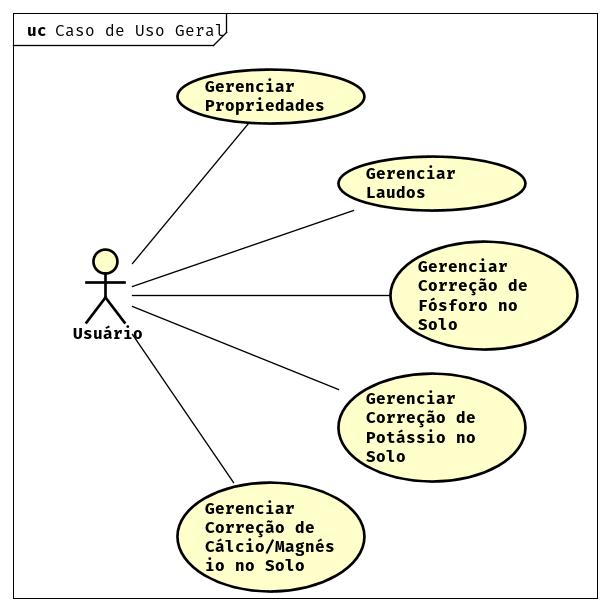
\includegraphics[width=13cm]{dados/figuras/casouso.jpg}
    \label{fig:diagramaCasoUso}
    \fonte{Autoria própria}
\end{figure}

Os casos de uso estão intimamente relacionados aos requisitos funcionais enumerados na \autoref{rf:tabela} e que serão comentados nas subseções abaixo.

\subsubsection{Caso de Uso - Gerenciar propriedades}
\label{sec:titSecCasoUsoPropriedades}

O Caso de Uso "Gerenciar propriedades" está relacionado ao requisito funcional RF001. Um propriedade representa uma área pertencente à um agricultor, como um sítio ou fazenda. Cada propriedade possui uma ou várias partições ou talhões, que será analisada, sendo assim, de suma importância para o funcionamento da aplicação. Como um produtor pode ter várias áreas analisadas em uma propriedades, faz-se necessário a criação de uma entidade no sistema.

\subsubsection{Caso de Uso - Gerenciar laudos}
\label{sec:titSecCasoUsoLaudos}

O caso de uso "Gerenciar laudos" referencia os RF02 a RF06. O laudo técnico do solo representa os indicadores de nutrientes do solo de um determinado talhão. Um talhão pode ser analisado diversas vezes. Por isso é importante que este laudo seja gerenciável como uma entidade na aplicação.

\subsubsection{Caso de Uso - Gerenciar correção de fósforo no solo}
\label{sec:titSecCasoUsoFosforo}

O caso de uso "Gerenciar correção de fósforo no solo" referencia os RF07 a RF09. As variáveis de correção do solo são: fonte de corretivo, eficiência, custo por tonelada. As fontes de corretivo possuem um valor padrão, que o usuário poderá editar no momento da realização do cálculo pois um determinado corretivo pode ser vendido com o mesmo nome mas ter propriedades diferentes. Por isso é necessário tornar gerenciável.

\subsubsection{Caso de Uso - Gerenciar correção de potássio no solo}
\label{sec:titSecCasoUsoPotassio}

O caso de uso "Gerenciar correção de potássio no solo" referencia os RF10 a RF12. Caso a saturação de bases fique além do ideal, é possível alterar o percentual desejado de potássio na CTC. Também deve ser possível o usuário alterar o valor em R\$/ton da fonte de potássio.

\subsubsection{Caso de Uso - Gerenciar correção do cálcio e magnésio no solo}
\label{sec:titSecCasoUsoCalcioMagnesio}

O caso de uso "Gerenciar correção do cálcio e magnésio no solo" referencia os RF13 a RF25. Caso a saturação de bases fique além do necessário, o usuário do sistema poderá corrigir o percentual de cálcio desejado na CTC. Além disso, também deve ser possível o usuário alterar o valor padrão do PRNT do corretivo, bem como o valor em R\$/ton.
\clearpage

\section{Diagrama de Classes}
\label{sec:titSecDiagClasse}

O Diagrama de Classes, segundo \cite{guedes2018uml}, define a estrutura das classes utilizadas pelo sistema, determinando os atributos e métodos que cada classe tem, além de estabelecer como as classes se relacionam e trocam informações entre si. A aplicação desse diagrama no sitema em questão pode ser vista na \autoref{fig:diagramaClasse}.

\begin{figure}[H]
    \centering
    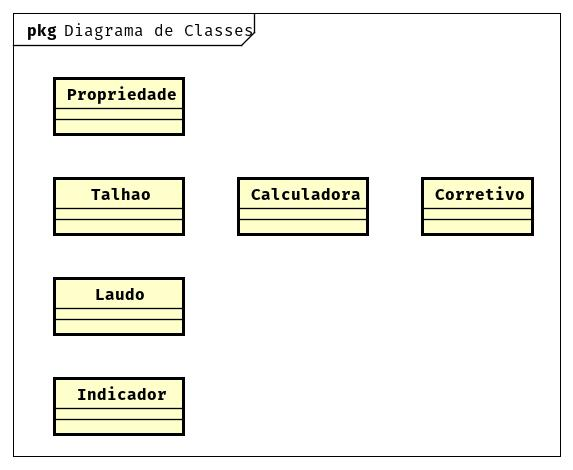
\includegraphics[width=13cm]{./dados/analise/diagramaclasse.jpg}
    \caption{Diagrama de Classes}
    \label{fig:diagramaClasse}
\end{figure}
\clearpage

\section{Projeto de Banco de Dados}
\label{sec:titSecBancoDados}

Segundo \cite{silberschatz2006sistema}, o objetivo do projeto de Banco de Dados é a construção de um conjunto de estruturas que permitam a representação de um dado de forma não redundante e que esse dado possa ser recuperado de forma simples. Este processo geralmente passa em diferentes níveis de abstração. Primeiramente, inicia-se com o entendimento do problema, para depois seguir por diferentes fases de modelagem, até chegar à implementação. Nesse processo, um modelo considerado padrão para a etapa inicial de modelagem é o entidade-relacionamento (ER) \cite{heuser2009projeto}.

\subsection{Diagrama de Entidade-Relacionamento}
\label{sec:titSecDiagER}

A modelagem entidade-relacionamento é a mais utilizada e difundida técnica de modelagem de dados. Nesta técnica, o modelo de dados é representado por meio de um modelo entidade-relacionamento (modelo ER). Comumente, o modelo ER é representado graficamente por meio de um diagrama entidade-relacionamento (DER) \cite{heuser2009projeto}.

A \autoref{fig:diagramaer} representa o DER do projetado neste documento.

\begin{figure}[H]
    \centering
    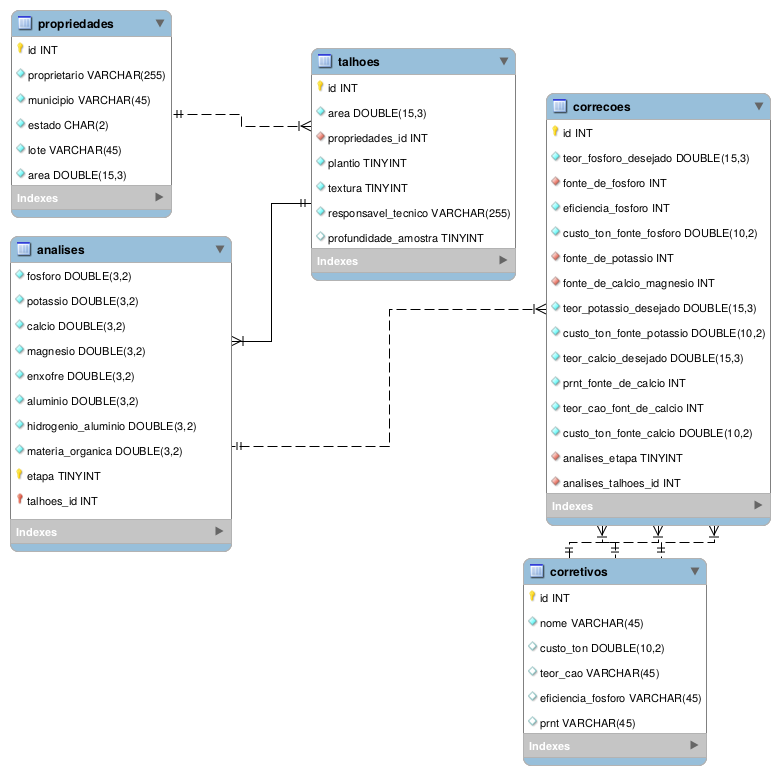
\includegraphics[width=13cm]{./dados/analise/diagramaer.png}
    \caption{Diagrama Entidade-Relacionamento}
    \label{fig:diagramaer}
\end{figure}

\subsection{Dicionário de Dados}
\label{sec:titSecDiagERDicionario}

\begin{landscape}
    \subsubsection{Tabela de Propriedades}
    \label{sec:titSubSecPropriedades}

    \begin{table}[H]
        \centering
        \caption[Tabela \textbf{propriedades}]{Na tabela propriedades ficarão armazenados os dados referentes à propriedade.
            \label{tab:tabela-er-propriedades}}
        \begin{tabular}{|p{4cm}|p{3cm}|p{2cm}|p{1cm}|p{2cm}|p{8cm}|}
            \hline
            Atributo     & Classe       & Domínio  & Bytes & Restrição & Descrição            \\\hline
            id           & Determinante & Numérico & 4     & PK, AI    &                      \\\hline
            proprietario & Simples      & Texto    & 255   & NN        & Nome do proprietário \\\hline
            municipio    & Simples      & Texto    & 255   & NN        & e.g. Dois Vizinhos   \\\hline
            estado       & Simples      & Texto    & 2     & NN        & e.g. PR              \\\hline
            lote         & Simples      & Texto    & 20    & NN        & e.g Q-103            \\\hline
            area         & Simples      & Numérico & 255   & NN        & Em metros quadrados  \\\hline
        \end{tabular}
    \end{table}

    \subsubsection{Tabela de Talhões}
    \label{sec:titSubSecTalhoes}

    \begin{table}[H]
        \centering
        \caption[Tabela \textbf{talhões}]{Na tabela talhões serão armazenados os dados referentes aos talhões da propriedade.
            \label{tab:tabela-er-talhoes}}
        \begin{tabular}{|p{4cm}|p{3cm}|p{2cm}|p{1cm}|p{2cm}|p{8cm}|}
            \hline
            Atributo              & Classe       & Domínio    & Bytes & Restrição & Descrição                        \\\hline
            id                    & Determinante & Numérico   & 4     & PK, AI    &                                  \\\hline
            area                  & Simples      & Numérico   & 10    & NN        & Em metros quadrados              \\\hline
            propriedades\_id      & Composto     & Numérico   & 255   & FK, NN    & Referência à tabela propriedades \\\hline
            plantio               & Simples      & Enumeravel & 1     & NN        & e.g. 1 (Plantio Direto)          \\\hline
            textura               & Simples      & Enumeravel & 1     & NN        & e.g. 2 (Textura Média)           \\\hline
            responsavel\_tecnico  & Simples      & Texto      & 255   & NN        & e.g. Pedro Cecere Filho          \\\hline
            profundidade\_amostra & Simples      & Numérico   & 255   &           & Em centímetros                   \\\hline
        \end{tabular}
    \end{table}

    \subsubsection{Tabela de Análises}
    \label{sec:titSubSecAnalises}

    \begin{table}[H]
        \centering
        \caption[Tabela \textbf{análises}]{Na tabela análises serão armazenados os dados do laudo técnico referente ao talhão.
            \label{tab:tabela-er-analises}}
        \begin{tabular}{|p{4cm}|p{3cm}|p{2cm}|p{1cm}|p{2cm}|p{8cm}|}
            \hline
            Atributo             & Classe       & Domínio  & Bytes & Restrição & Descrição                          \\\hline
            fosforo              & Simples      & Numérico & 4     & NN        & centimol de carga/decimetro cúbico \\\hline
            potassio             & Simples      & Numérico & 4     & NN        & centimol de carga/decimetro cúbico \\\hline
            calcio               & Simples      & Numérico & 4     & NN        & centimol de carga/decimetro cúbico \\\hline
            magnesio             & Simples      & Numérico & 4     & NN        & centimol de carga/decimetro cúbico \\\hline
            enxofre              & Simples      & Numérico & 4     & NN        & centimol de carga/decimetro cúbico \\\hline
            aluminio             & Simples      & Numérico & 4     & NN        & centimol de carga/decimetro cúbico \\\hline
            hidrogenio\_aluminio & Simples      & Numérico & 4     & NN        & centimol de carga/decimetro cúbico \\\hline
            materia\_organica    & Simples      & Numérico & 4     & NN        & centimol de carga/decimetro cúbico \\\hline
            etapa                & Determinante & Numérico & 4     & PK, AI    &                                    \\\hline
            talhoes\_id          & Composto     & Numérico & 4     & PK, FK    & Referência à tabela talhoes        \\\hline
        \end{tabular}
    \end{table}

    \subsubsection{Tabela de Correções}
    \label{sec:titSubSecAnalises}

    \begin{table}[H]
        \centering
        \caption[Tabela \textbf{Correções}]{Na tabela Correções serão armazenados os dados úteis para o cálculo do equilíbrio e correção do solo.
            \label{tab:tabela-er-correcoes}}
        \begin{tabular}{|p{4cm}|p{3cm}|p{2cm}|p{1cm}|p{2cm}|p{8cm}|}
            \hline
            Atributo                    & Classe       & Domínio  & Bytes & Restrição & Descrição                         \\\hline
            id                          & Determinante & Numérico & 4     & PK, AI    &                                   \\\hline
            teor\_fosforo\_desejado     & Simples      & Numérico & 1     & NN        & em percentual                     \\\hline
            fonte\_de\_fosforo          & Composto     & Numérico & 4     & NN        & em referência à tabela corretivos \\\hline
            eficiencia\_fosforo         & Simples      & Numérico & 1     & NN        & em percentual                     \\\hline
            custo\_ton\_fonte\_fosforo  & Simples      & Numérico & 8     & NN        & em R\$/tonelada                   \\\hline
            fonte\_de\_potassio         & Composto     & Numérico & 4     & NN        & em referência à tabela corretivos \\\hline
            fonte\_de\_calcio\_magnesio & Composto     & Numérico & 4     & NN        & em referência à tabela corretivos \\\hline
            teor\_potassio\_desejado    & Simples      & Numérico & 1     & NN        & em percentual                     \\\hline
            custo\_ton\_fonte\_potassio & Simples      & Numérico & 8     & NN        & em R\$/tonelada                   \\\hline
            teor\_calcio\_desejado      & Simples      & Numérico & 1     & NN        & em percentual                     \\\hline
            prnt\_fonte\_de\_calcio     & Simples      & Numérico & 1     & NN        & em percentual                     \\\hline
            teor\_cao\_font\_de\_calcio & Simples      & Numérico & 1     & NN        & em percentual                     \\\hline
            custo\_ton\_fonte\_calcio   & Simples      & Numérico & 8     & NN        & em R\$/tonelada                   \\\hline
            analises\_etapa             & Composto     & Numérico & 4     & FK        & Referência à tabela talhoes       \\\hline
            analises\_talhoes\_id       & Composto     & Numérico & 4     & FK        & Referência à tabela talhoes       \\\hline
        \end{tabular}
    \end{table}

    \subsubsection{Tabela de Correções}
    \label{sec:titSubSecAnalises}

    \begin{table}[H]
        \centering
        \caption[Tabela \textbf{Corretivos}]{Na tabela Corretivos serão armazenados os dados padrões acerca dos corretivos.
            \label{tab:tabela-er-correcoes}}
        \begin{tabular}{|p{4cm}|p{3cm}|p{2cm}|p{1cm}|p{2cm}|p{8cm}|}
            \hline
            Atributo            & Classe       & Domínio  & Bytes & Restrição & Descrição       \\\hline
            id                  & Determinante & Numérico & 4     & PK, AI    &                 \\\hline
            nome                & Simples      & Texto    & 255   & NN        & em percentual   \\\hline
            custo\_ton          & Simples      & Numérico & 8     &           & em R\$/tonelada \\\hline
            teor\_cao           & Simples      & Numérico & 1     &           & em percentual   \\\hline
            eficiencia\_fosforo & Simples      & Numérico & 1     &           & em percentual   \\\hline
            prnt                & Simples      & Numérico & 1     &           & em percentual   \\\hline
        \end{tabular}
    \end{table}

\end{landscape}
\clearpage

\subsection{Diagrama de Implantação}
\label{sec:titSecDiagDeploy}

O Diagrama de Implantação determina as necessidades de \textit{hardware} do sistema, as características físicas como servidores, estações, topologias e protocolos de comunicação \cite{guedes2018uml}, destacando todos as necessidades físicas no qual o sistema deverá ser executado. Também é mostrado como será a distribuição dos módulos do sistema nos momentos onde a aplicação estará sendo executada em diferentes servidores.

\begin{figure}[H]
    \centering
    \caption{Representação do Diagrama de Implantação}
    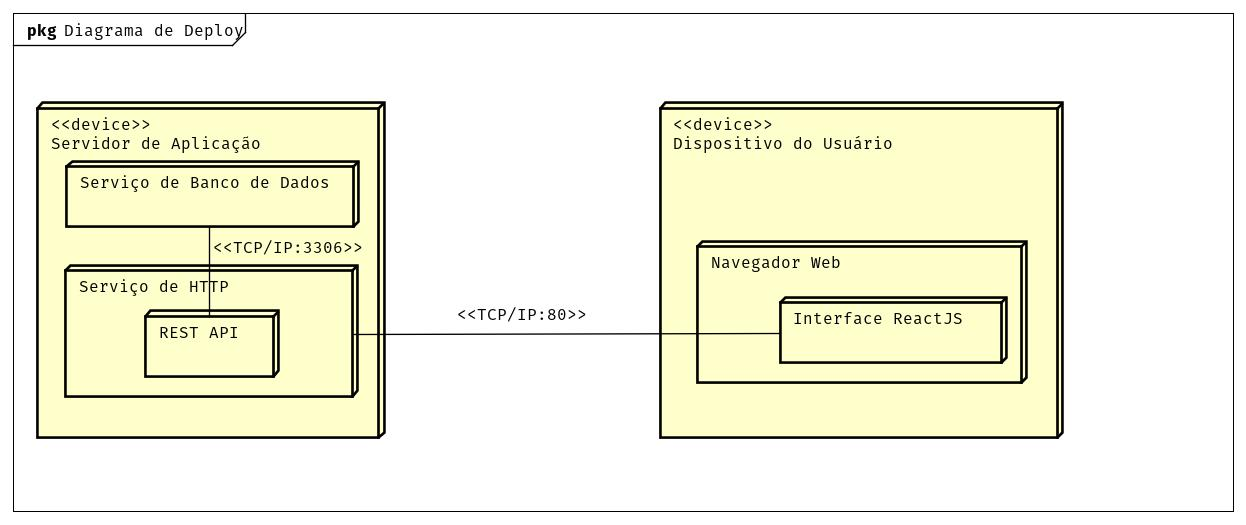
\includegraphics[width=13cm]{dados/figuras/diagramadeploy.jpg}
    \label{fig:diagramaDeploy}
    \fonte{Autoria própria}
\end{figure}

A \autoref{fig:diagramaDeploy} mostra a aplicação desse conceito no projeto. Nela é possível observar a distribuição do sistema em dois nós principais. O primeiro é o servidor de aplicação, que faz o encapsulamento do servidor Apache. Nesse mesmo servidor é possível observar a presença de um servidor MySQL, o qual será responsável por armazenar os dados do sistema e só receberá acessos locais.
O outro nó, representa o lado do cliente da aplicação, responsável pelas chamadas ao recursos contidos no servidor \textit{web} por meio de requisições Ajax, por meio do protocolo HTTP.

\clearpage

\section{PROTÓTIPOS DE TELA}
\label{sec:titSecPrototipos}

% Os protótipos de tela são uma versão inicial de um sistema. Eles são usados, dentre outras razões, para descobrir mais sobre um problema e suas possíveis soluções. O desenvolvimento rápido e iterativo do protótipo previne gastos desnecessários e custos controlados e os \textit{stakeholders} podem fazer usos pontuais de partes do sistema desde o início do desenvolvimento \citeonline{Sommerville10}.

% Além disso, os protótipos podem ajudar na antecipação de mudanças que podem ser requisitadas.
% Para o presente projeto foram desenvolvidas três interfaces para dois tamanhos diferentes de tela, simulando um dispositivo de tela maior (\textit{desktop}, \textit{tablet}) e outro para telas menores (\textit{smartphones}).

% O modelo de prototipação é ideal quando o cliente não tem os requisitos muito bem definidos, que é o caso do aplicativo estudado neste documento. Visto que os requisitos foram levantados com base em uma planilha, conforme explicado anteriormente na \autoref{sub:processo}.

Nas próximas subseções serão exibidos os protótipos de tela para três principais operações que o usuário poderá realizar no sistema, que são a tela que o usuário é enviado após fazer o \textit{login}, a tela para criação de um novo recurso no sistema e a tela de exibição de um recurso.

\subsection{Protótipos para tela inicial do sistema}
\label{sec:titSecPrototiposHome}

As Figuras \ref{fig:prototipo_home_desk} e \ref{fig:prototipo_home_mobile}, representam a visão da página inicial do sistema, que será exibida após o login do usuário. É possível observar que logo na parte superior, existirão quadros informativos sobre a quantidade de propriedades assistidas, quantidade de cidades atendidas e a área em hectares que foram tratadas (ou corrigidas). Logo abaixo serão exibidas as últimas correções realizadas pelo usuário.

\begin{figure}[H]
    \centering
    \caption{Página que será exibida após o login do usuário na visão de um dispositivo \textit{desktop}}
    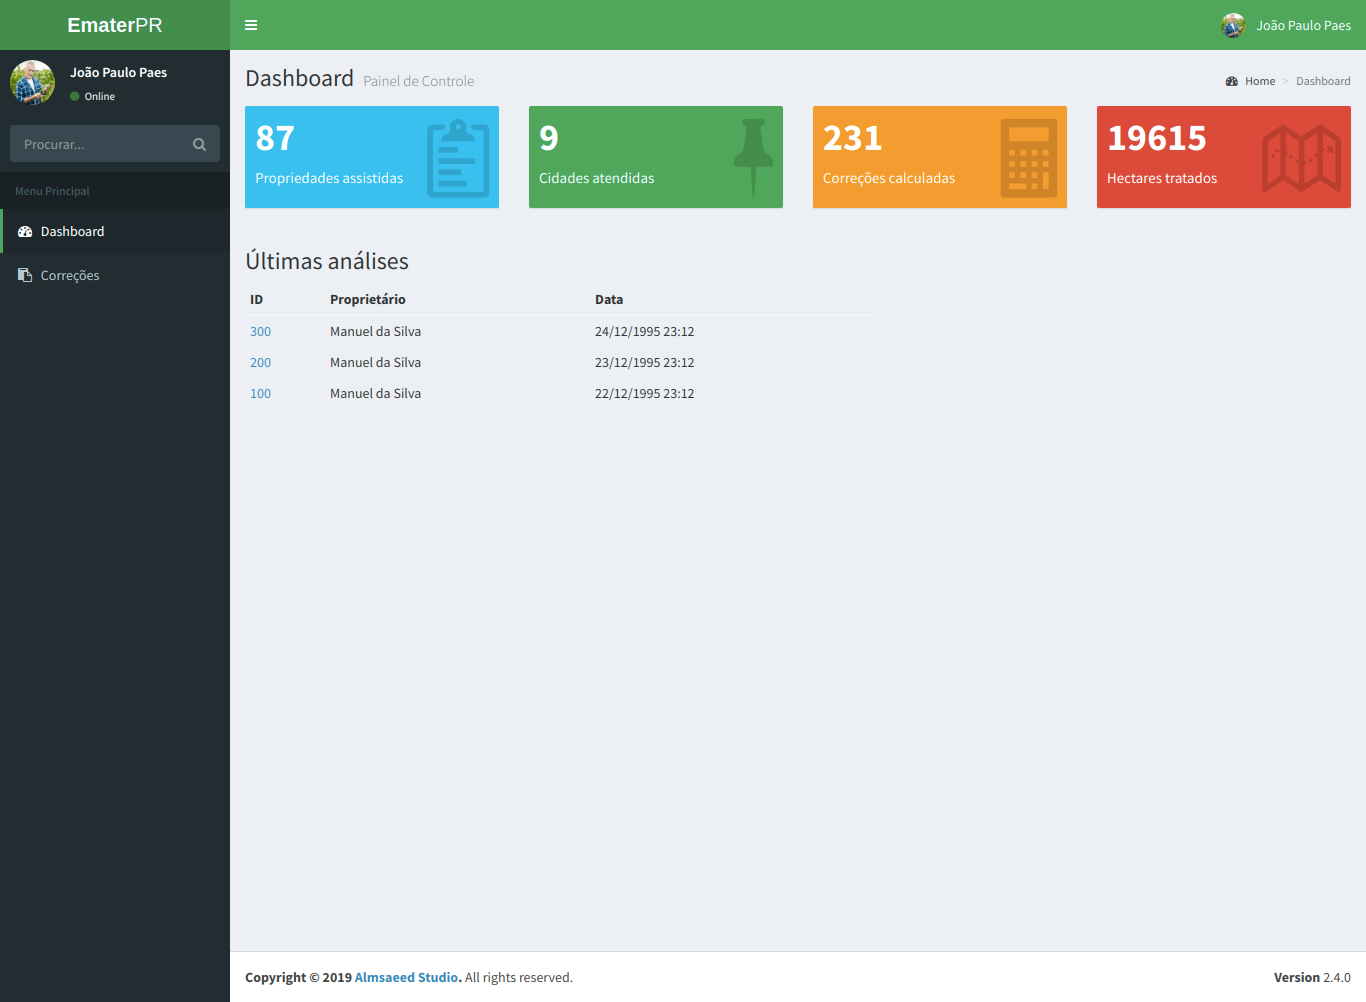
\includegraphics[width=13cm]{./dados/figuras/prototipos/home_desktop.png}
    \label{fig:prototipo_home_desk}
    \fonte{Autoria própria}
\end{figure}

\begin{figure}[H]
    \centering
    \caption{Página que será exibida após o login do usuário na visão de um dispositivo \textit{mobile}}
    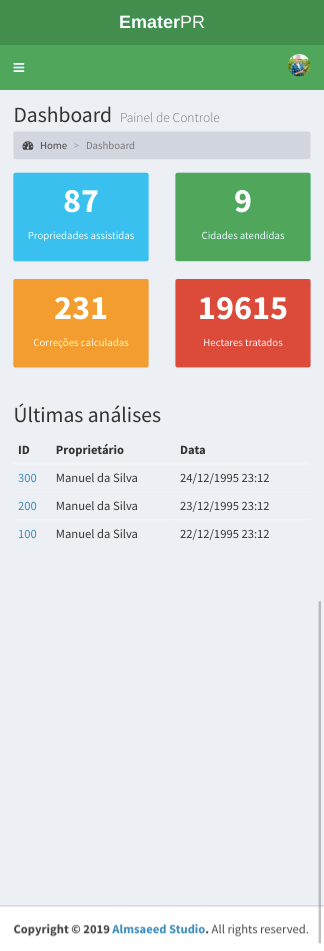
\includegraphics[width=6cm]{./dados/figuras/prototipos/home_mobile.png}
    \label{fig:prototipo_home_mobile}
    \fonte{Autoria própria}
\end{figure}

\subsection{Protótipos para tela de cadastro de informação}
\label{sec:titSecPrototiposCreate}

A tela de cadastro de informações foi pensada para ser intuitiva e reativa como a planilha. Como é um formulário grande, será divido em \textit{steps} que serão exibidos na parte superior do formulário, tendo a descrição do que deve ser feito naquele \textit{step} logo abaixo. Já o formulário propriamente dito terá uma interface reativa, que lembra a planilha.

No exemplo mostrado nas Figuras \ref{fig:prototipo_create_desk} e \ref{fig:prototipo_create_mobile}, é possível observar que caso o valor de um campo esteja no intervalo ideal, este deverá ter a sua \textit{label} e o contorno destacados em verde. Enquanto se o valor estiver fora do intervalo, em âmbar. 

\begin{figure}[H]
    \centering
    \caption{Criação de recurso na visão de um dispositivo \textit{desktop}}
    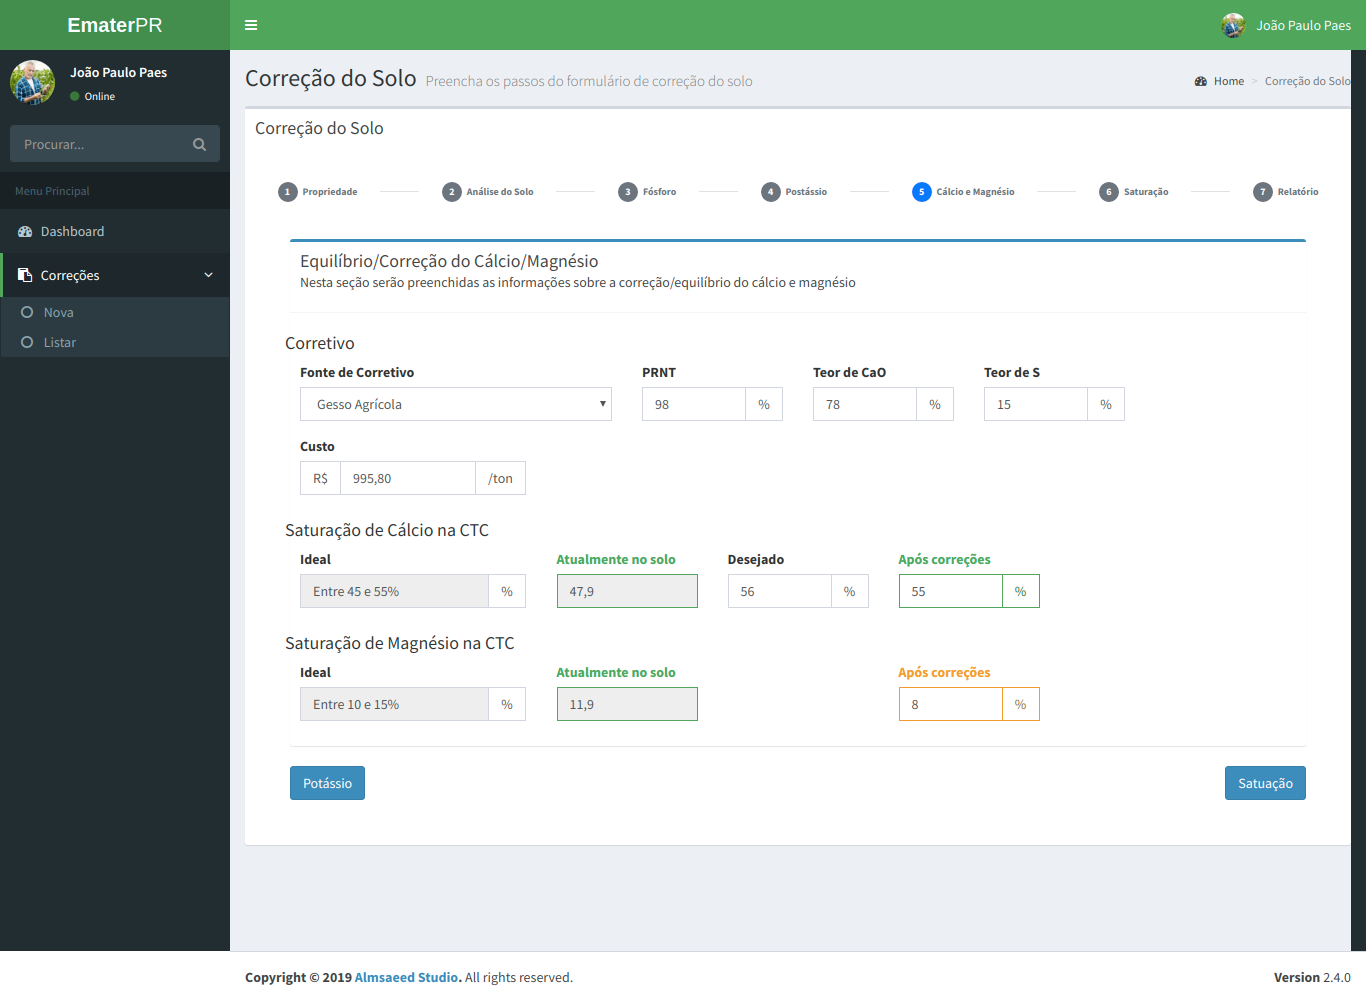
\includegraphics[width=13cm]{./dados/figuras/prototipos/create_desktop.png}
    \label{fig:prototipo_create_desk}
    \fonte{Autoria própria}
\end{figure}

\begin{figure}[H]
    \centering
    \caption{Criação de recurso na visão de um dispositivo \textit{mobile}}
    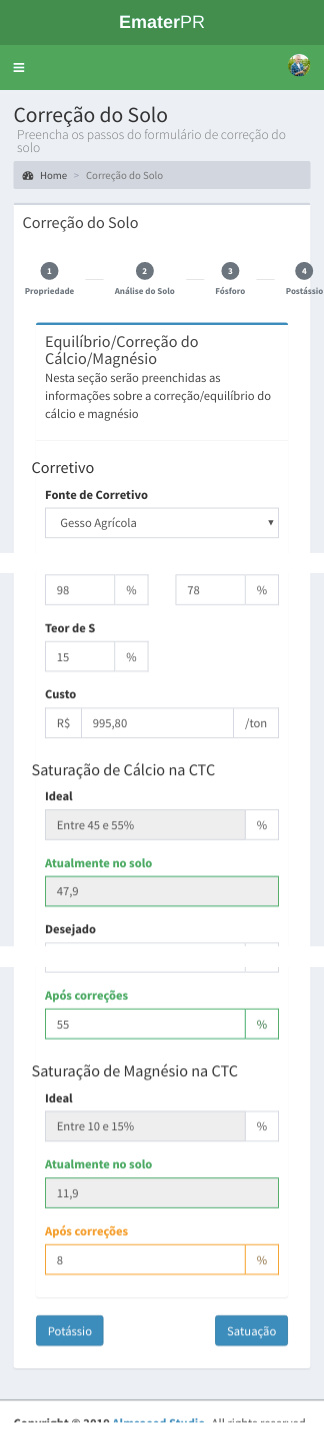
\includegraphics[width=6cm]{./dados/figuras/prototipos/create_mobile.png}
    \label{fig:prototipo_create_mobile}
    \fonte{Autoria própria}
\end{figure}


\subsection{Protótipos para tela de exibição de informação}
\label{sec:titSecPrototiposShow}

A tela de exibição da informação também seguirá o modelo de \textit{steps}. Ela deverá ser dividia em 3 colunas para representar os três estados da correção do solo: naquele momento, desejado e após as correções. É possível notar que os textos deverão estar coloridos de acordo com o caso no qual se encaixa. Acima do valor, amarelo. Abaixo do valor, vermelho. No intervalo, verde.

\begin{figure}[H]
    \centering
    \caption{Visualização de recurso na visão de um dispositivo \textit{desktop}}
    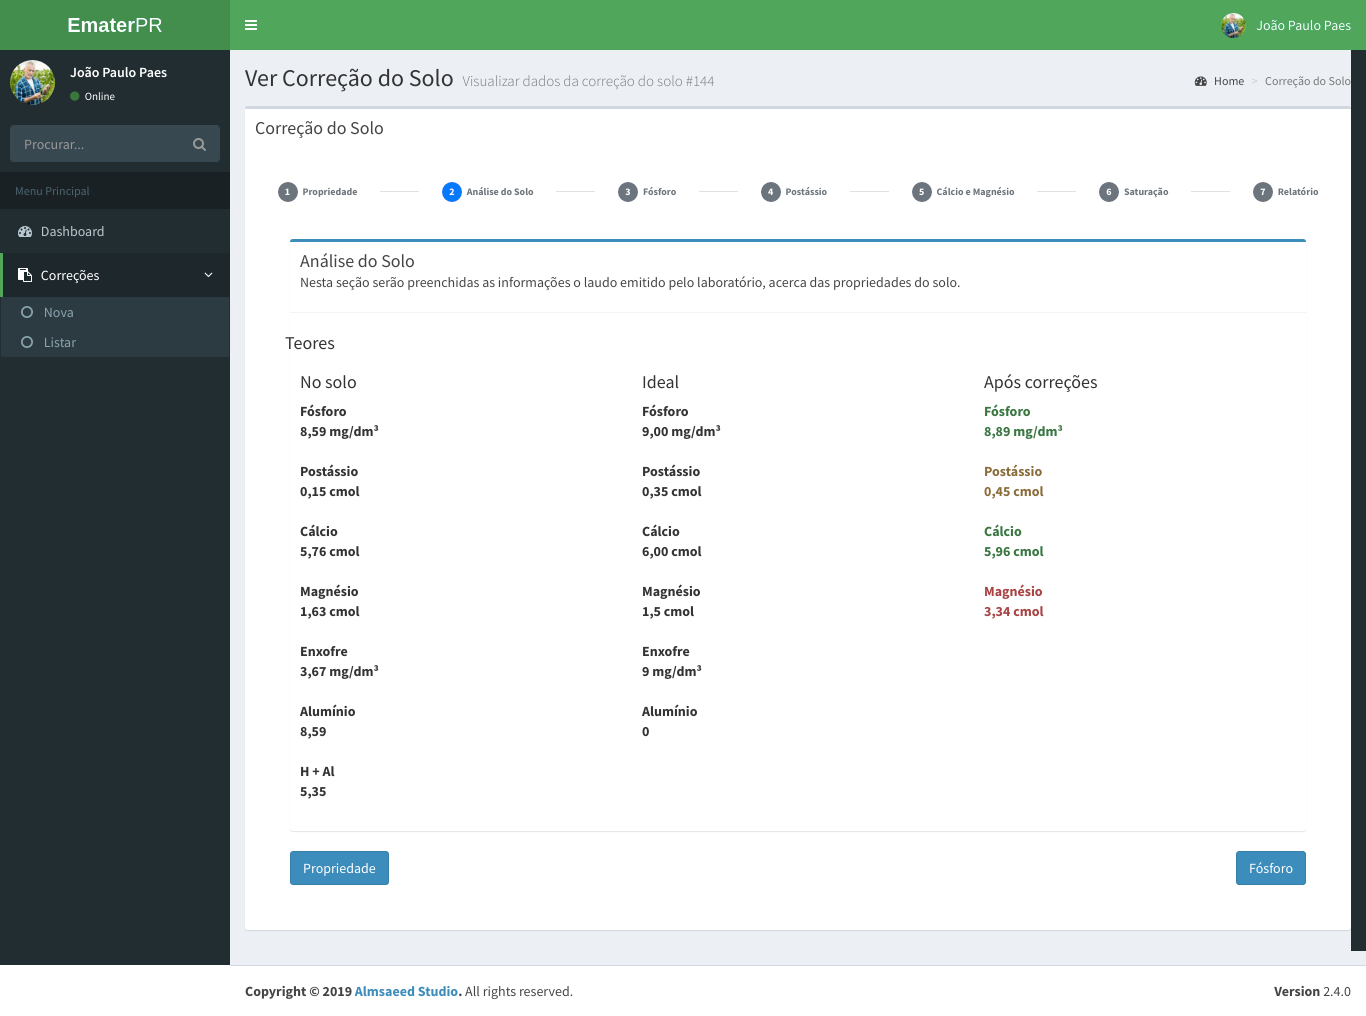
\includegraphics[width=13cm]{./dados/figuras/prototipos/show_desktop.png}
    \label{fig:prototipo_show_desk}
    \fonte{Autoria própria}
\end{figure}

\begin{figure}[H]
    \centering
    \caption{Visualização de recurso na visão de um dispositivo \textit{mobile}}
    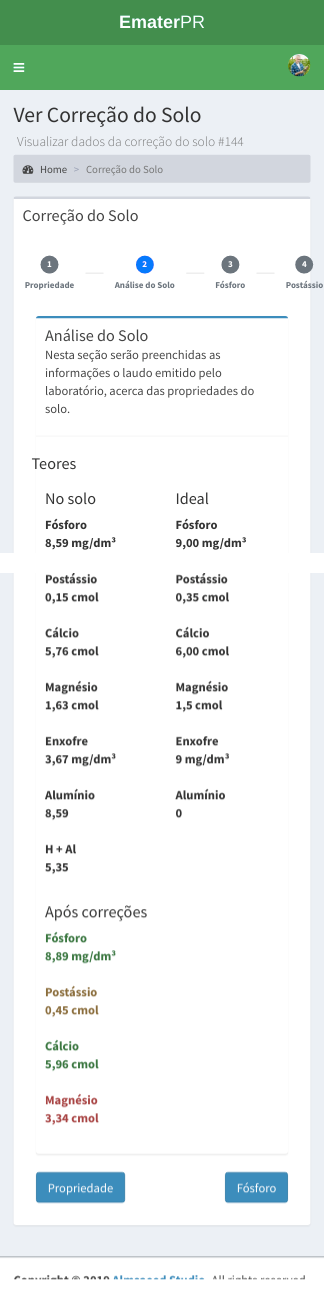
\includegraphics[width=6cm]{./dados/figuras/prototipos/show_mobile.png}
    \label{fig:prototipo_show_mobile}
    \fonte{Autoria própria}
\end{figure}
\clearpage


\chapter{CRONOGRAMA DO PROJETO}

% \section{CRONOGRAMA DO PROJETO}
% \label{sec:cronograma}

O gráfico do abaixo demonstra a distribuição das atividades do projeto em relação ao tempo. A data da primeira reunião com o professor orientador foi considerada a data inicial do cronograma, na qual foi definido o tema a ser desenvolvido. A duração de cada atividade está na unidade de dias.

\begin{landscape}

    \begin{ganttchart}
        [
            y unit title=0.4cm,
            y unit chart=0.5cm,
            vgrid,hgrid,
            title height=1,
            bar/.style={draw,fill=green},
            bar incomplete/.append style={fill=yellow!50},
            bar height=0.7
        ]{1}{36}

        \gantttitle{Junho}{6}
        \gantttitle{Julho}{5}
        \gantttitle{Agosto}{5}
        \gantttitle{Setembro}{5}
        \gantttitle{Outubro}{5}
        \gantttitle{Novembro}{5}
        \gantttitle{Dezembro}{5} \\

        \gantttitlelist{1,...,6}{1}
        \gantttitlelist{1,...,5}{1}
        \gantttitlelist{1,...,5}{1}
        \gantttitlelist{1,...,5}{1}
        \gantttitlelist{1,...,5}{1}
        \gantttitlelist{1,...,5}{1}
        \gantttitlelist{1,...,5}{1} \\

        \gantttitlelist{1,...,36}{1} \\

        \ganttbar{Desenvolvimento da Interfaces}{2}{17} \\

        \ganttbar{Desenvolvimento da API Rest}{4}{20} \\

        \ganttbar{Correções no Documento}{5}{5}
        \ganttbar{}{10}{10}
        \ganttbar{}{15}{15}
        \ganttbar{}{20}{20}
        \ganttbar{}{24}{30}\\

        \ganttbar{Entrega do Documento}{31}{30} \\

        \ganttbar{Validação pelo técnico}{5}{4}
        \ganttbar{}{10}{9}
        \ganttbar{}{15}{14}
        \ganttbar{}{20}{19} \\

        \ganttbar{Entrega parcial}{7}{6}
        \ganttbar{}{12}{11}
        \ganttbar{}{17}{16}
        \ganttbar{}{22}{21} \\

        \ganttbar{Implantação}{22}{24} \\

        \ganttbar{Testes exploratórios pelo cliente}{25}{29} \\
        \ganttbar{Correção de bugs}{25}{29} \\

    \end{ganttchart}

\end{landscape}